\documentclass[11pt]{article}
\usepackage{geometry}
\usepackage{float}
\usepackage{amsmath}
\usepackage{circuitikz}
\usepackage{amssymb}
\usepackage{mathtools}
\usepackage{tikz}
\usepackage{tikz-3dplot}
\usepackage{cite}
\usepackage{url}
\usetikzlibrary{chains}
\usetikzlibrary{decorations.pathmorphing,calc,positioning,arrows.meta}
\usetikzlibrary{positioning,shapes,arrows.meta}
\usetikzlibrary{circuits.ee.IEC}
\usepackage{graphicx}
\usepackage{xcolor}
\usepackage{parskip}

\definecolor{Mcolor}{HTML}{000000}
\definecolor{Mproj}{HTML}{505050}
\definecolor{Bzerocolor}{HTML}{DA4333}
\definecolor{Bzerocircle}{HTML}{989952}
\definecolor{Bonecolor}{HTML}{FE9920}
\definecolor{Bonecircle}{HTML}{456C81}

\DeclarePairedDelimiter{\set}{\{}{\}}

\title{Pulsed Nuclear Magnetic Resonance}
\author{Spandan Suthar and Antoni Gonzalez}
\date{January 21, 2026}

\geometry{margin=1in}

\begin{document}

\maketitle

\section{Introduction and Background}

Nuclear magnetic resonance (NMR) involves subjecting particles to
large stationary magnetic
fields and measuring the particles' responses to additional, smaller
oscillatory magnetic fields supplied by closely controlled
radiofrequency (RF) signals \cite{mel}. The
resonant frequencies of particles
and parameters of the particles'
response behaviors are characteristic of the particle, its
surrounding magnetic
environment (e.g., magnetic field strength), and its chemical
environment (e.g., bonds and neighboring atoms) \cite{spect, harris, mel}.
This uniqueness allows for the identification of molecular structures,
the selective manipulation of spins in complex systems, and
the localization of spins through their responses'
dependence on the strength of an applied magnetic
field \cite{spect, harris, mel}. Notable direct applications include
magnetic resonance
imaging (MRI), which leverages localization abilities, and nuclear
magnetic resonance spectroscopy, which utilizes
the characteristic nature
of particle responses for compound identification \cite{spect,
harris, mel}. By placing
particles in very predictable situations and by
investigating their reversible and irreversible relaxations
in response to RF pulses of precise length and frequency, pulsed NMR
(pNMR) experiments collect useful reference
information for identifying particles or substances, produce data
corroborating physicists'
understanding of how
many-spin systems act in aggregate, and demonstrate the precision with which
particles can be manipulated as tools to accomplish larger scientific
and medical ends \cite{mel}.

This pNMR experiment utilizes RF pulses to place
nucleus dipoles of various solutions in higher-energy states, then
measures the times taken for the independent relaxations of the
solution's net magnetization vector's longitudinal and transverse
components relative to a large static magnetic field.

Consider a number of
nuclei suspended in a fluid, subject to a static external
magnetic field $\vec{B}_0$ defining a $z$-axis and an orthogonal
$x$-$y$-plane (transverse plane). Each proton has an
intrinsic angular momentum--its spin--to which a parallel intrinsic magnetic
dipole moment $\vec{\mu}$ is associated.
A magnetic dipole placed in a static magnetic field
precesses about the magnetic
field with a Larmor frequency \cite{young, knight, harris};
thus, each proton's magnetic
dipole moment
precesses about
$\vec{B}_0$ with phases that are initially uniformly distributed. The
state in which a proton's magnetic dipole moment is aligned with
$\vec B_0$ is of lower energy than the anti-aligned state
\cite{young, knight, harris}, causing an
excess of protons with a positive spin $z$-component. This results in a
net magnetization vector $\vec{M}$ initially parallel to $\vec{B}_0$, as
shown in Figure \ref{fig:dipole_angular_momentum_3d}.

When a secondary
magnetic field $\vec{B}_1$ is applied parallel to the transverse
plane, $\vec M$ briefly precesses about $\vec{B}_1$ and accrues a nonzero
angle $\alpha$ from the $z$-axis as each nucleus gains the same
additional nonzero transverse component in expectation \cite{sakurai,
harris, mel}. As
$\vec M$ is no longer parallel to
$\vec{B}_0$, $\vec M$ also precesses about $\vec{B}_0$ with a precession
angle $\beta$ and a Larmor frequency $\omega_0$ \cite{young, knight,
harris}. In this state, the
longitudinal and transverse components of $\vec M$ ($\vec M_z$ and
$\vec M_{xy}$) are both nonzero.
To maximize the growth rate of $\alpha$, $\vec B_1$ must rotate about the
$z$-axis at frequency $\omega_0$ defining a consistent transverse axis of
precession for $\vec M$ within its frame of precession about $\vec B_0$. Thus,
the condition for causing a sustained growth of $\alpha$ is a resonance
condition $\omega_1 = \omega_0$ \cite{young, knight}, where $\omega_1$ is the
frequency of $\vec B_1$'s motion in the transverse plane.

In practice, the necessary $\vec B_1$ is produced by a linearly
polarized oscillatory magnetic field $\vec B_{RF}$  of frequency
$\omega_1$, usually supplied by a radio frequency (RF) coil. Such a
time-dependent field is physically indistinguishable
from applying two counter-rotating circularly polarized magnetic
fields of equal strength
and frequency $\omega_1$: $\vec B_{RF} = \vec B_1 + \vec B_1'$. When
the resonance condition $\omega_1 = \omega_0$ is met, $\vec B_{1}'$'s
motion is significantly
far from being stationary in the precession frame of $\vec M$ about $\vec
B_0$, making its effect on $\vec M$ negligible relative to $\vec B_1$
and allowing the approximation $\vec B_{RF} \approx
\vec B_1$. This yields precisely the rotating $\vec B_1$ necessary
for the sustained growth of $\alpha$.

\vspace{1em}

\begin{figure}[H]
  \centering
  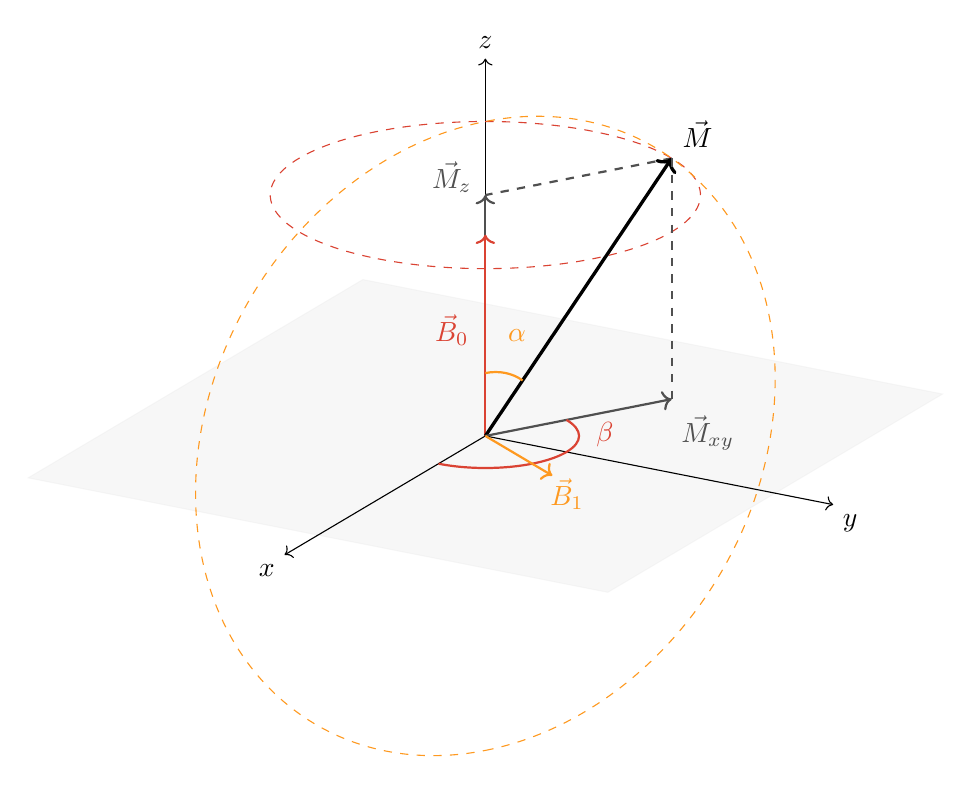
\begin{tikzpicture}[scale=1.7]
    % Set viewing angles
    \tdplotsetmaincoords{70}{120}
    \begin{scope}[tdplot_main_coords]
      % Define the angle for L vector (in spherical coordinates)
      \def\theta{40}
      \def\phi{150}
      \def\Lradius{2.5}
      \def\muradius{1.3}
      % Calculate coordinates
      \pgfmathsetmacro{\Lx}{\Lradius*sin(\theta)*cos(\phi)}
      \pgfmathsetmacro{\Ly}{\Lradius*sin(\theta)*sin(\phi)}
      \pgfmathsetmacro{\Lz}{\Lradius*cos(\theta)}
      \pgfmathsetmacro{\mux}{\muradius*sin(\theta)*cos(\phi)}
      \pgfmathsetmacro{\muy}{\muradius*sin(\theta)*sin(\phi)}
      \pgfmathsetmacro{\muz}{\muradius*cos(\theta)}

      % Calculate the radius of the circle in the xy-plane
      \pgfmathsetmacro{\LxyRadius}{sqrt(\Lx*\Lx + \Ly*\Ly)}

      % Draw the orthogonal plane (perpendicular to B) - FIRST for
      % proper layering
      \filldraw[gray!20, opacity=0.3] (-2.5,-2.5,0) -- (2.5,-2.5,0)
      -- (2.5,2.5,0) -- (-2.5,2.5,0) -- cycle;

      % Draw coordinate axes
      \draw[black,->] (0,0,0) -- (3,0,0) node[anchor=north east]{$x$};
      \draw[black,->] (0,0,0) -- (0,3,0) node[anchor=north west]{$y$};
      \draw[black,->] (0,0,0) -- (0,0,3) node[anchor=south]{$z$};

      % Projection of M onto the z-axis (drawn before B for proper layering)
      \draw[thick, dashed, Mproj] (\Lx,\Ly,\Lz) -- (0,0,\Lz);
      \draw[thick, Mproj, ->] (0,0,0) -- (0,0,\Lz);
      \node[Mproj] at (0.5,0,\Lz+0.3) {$\vec{M}_{z}$};

      % Vertical magnetic field vector along z-axis
      \draw[thick, Bzerocolor, ->] (0,0,0) -- (0,0,1.6);
      \node[Bzerocolor] at (0.5,0,1.0) {$\vec{B}_0$};

      % Draw the circle parallel to xy-plane passing through the tip of L
      \draw[dashed, Bzerocolor] (0,0,\Lz) circle (\LxyRadius);

      % Magnetization vector
      \draw[very thick, Mcolor, ->] (0,0,0) -- (\Lx,\Ly,\Lz) node[above
      right] {$\vec{M}$};

      % Projection of M onto the xy-plane
      \draw[thick, dashed, Mproj] (\Lx,\Ly,\Lz) -- (\Lx,\Ly,0);
      \draw[thick, Mproj, ->] (0,0,0) -- (\Lx,\Ly,0);
      \node[Mproj] at (\Lx+0.5,\Ly+0.6,0) {$\vec{M}_{xy}$};

      % Arc showing angle beta from x-axis to M_perp projection
      \pgfmathsetmacro{\betaAngle}{atan2(\Ly,\Lx)}
      \draw[thick, Bzerocolor] (0,0,0) + (0:0.7) arc (0:{\betaAngle}:0.7);
      \pgfmathsetmacro{\betaLabelAngle}{\betaAngle/2}
      \pgfmathsetmacro{\betaLabelX}{1.1*cos(\betaLabelAngle) - 0.75}
      \pgfmathsetmacro{\betaLabelY}{1.1*sin(\betaLabelAngle) - 0.3}
      \node[Bzerocolor] at (\betaLabelX,\betaLabelY,0) {$\beta$};

      % B_1 vector - orthogonal to M_xy in the xy-plane, first quadrant
      \pgfmathsetmacro{\Bnorm}{sqrt(\Lx*\Lx + \Ly*\Ly)}
      \pgfmathsetmacro{\BoneScale}{1.0}
      \pgfmathsetmacro{\BoneX}{\BoneScale*\Ly/\Bnorm}
      \pgfmathsetmacro{\BoneY}{-\BoneScale*\Lx/\Bnorm}
      \draw[thick, Bonecolor, ->] (0,0,0) -- (\BoneX,\BoneY,0);
      \node[Bonecolor] at (\BoneX+0.3,\BoneY+0.3,0) {$\vec{B}_1$};

      % Dashed circle centered at origin, in plane perpendicular to
      % B_1, passing through M
      % Calculate angle of B_1 and radius perpendicular to B_1
      \pgfmathsetmacro{\BoneAngle}{atan2(\BoneY,\BoneX)}
      \pgfmathsetmacro{\BoneNorm}{sqrt(\BoneX*\BoneX + \BoneY*\BoneY)}
      \pgfmathsetmacro{\MdotBone}{(\Lx*\BoneX + \Ly*\BoneY)/\BoneNorm}
      \pgfmathsetmacro{\MparallelX}{\MdotBone*\BoneX/\BoneNorm}
      \pgfmathsetmacro{\MparallelY}{\MdotBone*\BoneY/\BoneNorm}
      \pgfmathsetmacro{\MperpX}{\Lx - \MparallelX}
      \pgfmathsetmacro{\MperpY}{\Ly - \MparallelY}
      \pgfmathsetmacro{\MperpZ}{\Lz}
      \pgfmathsetmacro{\radiusPerpToBone}{sqrt(\MperpX*\MperpX +
      \MperpY*\MperpY + \MperpZ*\MperpZ)}
      \tdplotsetrotatedcoords{\BoneAngle}{90}{0}
      \tdplotdrawarc[tdplot_rotated_coords,dashed,Bonecolor]{(0,0,0)}{\radiusPerpToBone}{0}{360}{}{}

      % Arc showing angle between B and L
      % Draw the arc WITHOUT a label first
      \tdplotsetthetaplanecoords{\phi}
      \tdplotdrawarc[tdplot_rotated_coords,thick,Bonecolor]{(0,0,0)}{0.5}{0}{\theta}{}{}

      % Calculate a position for the alpha symbol
      \pgfmathsetmacro{\labelR}{0.8}
      \pgfmathsetmacro{\labelTheta}{\theta/2}
      \pgfmathsetmacro{\labelX}{\labelR*sin(\labelTheta)*cos(\phi)}
      \pgfmathsetmacro{\labelY}{\labelR*sin(\labelTheta)*sin(\phi)}
      \pgfmathsetmacro{\labelZ}{\labelR*cos(\labelTheta)}

      % Place the symbolic alpha instead of theta
      \node[Bonecolor] at (\labelX,\labelY,\labelZ) {$\alpha$};
    \end{scope}
  \end{tikzpicture}
  \caption{Diagram of $\vec M$, the net magnetization vector, as it
    precesses with angle $\beta$ about an external static magnetic field
    $\vec B_0$ and precesses with angle $\alpha$ about a secondary
    magnetic field $\vec B_1$ applied by an
    RF coil. Note that $\vec B_1$ is in the transverse plane and static
    within the precession frame of $\vec M$ about $\vec B_0$. $\vec
    M$ is projected onto the $z$ axis to produce
  $\vec M_z$ and the $xy$ plane to produce $\vec M_{xy}$.}
  \label{fig:dipole_angular_momentum_3d}
\end{figure}

The Larmor frequency
of these nuclei associated with precession about $\vec B_1$ results in the net
magnetization's $\omega_1$ and is given by $\omega_1 =
\frac{g_f \mu_N B_1}{\hbar} = \frac{d\alpha}{dt}$ \cite{sakurai,
harris, mel}. Therefore, $\alpha$ is
proportional to the lifetime $\Delta t_{B_1}$ and strength of $\vec B_1$:

\begin{equation}
  \alpha = \omega_1 \Delta t_{B_1} = \frac{g_f \mu_N B_1}{\hbar}
  \Delta t_{B_1}
  \label{eq:alpha}
\end{equation}

Because states with a larger $\vec M_z$ have a larger dot product
with $\vec B_0$, these states have a lower potential energy $U = -
\vec M \cdot \vec B_0 = - M_z B_0$ \cite{knight, young}. When $\vec B_1$ is no
longer applied, the system spontaneously
evolves in a manner that grows $\vec M_z$ along positive $z$, releasing
thermal energy
conceptualized as phonons
into the surrounding environment as the system's energy decreases \cite{kittel,
ashcroft_mermin}. This
interaction between $\vec M$
and the environment is
known as a spin-lattice relaxation \cite{mel}, characterized by a time
$T_1$ \cite{mel}:

\begin{equation}
  M_z(t) = M_z(0) \left(1 - 2 \cdot e^{- \frac{t}{T_1}} \right)
  \label{eq:spin_lattice_relaxation}
\end{equation}

Because it is orthogonal to $\vec B_0$, $\vec M_{xy}$ has no contribution to the
dot product with $\vec B_0$. Therefore, the component of $\vec M$ in
the transverse plane does not spontaneously decay in the same manner.
Instead, two transverse-component effects occur independently of the
longitudinal relaxation. The first is a reversible effect due to
spatial nonuniformities $\vec \Delta B_0(\vec r)$ of $\vec B_0$
\cite{mel}. These
make the Larmor frequency of each nucleus a function of position, causing
different linear rates of evolution of each nucleus's precession
angle--which reach values $\beta_i$ after time $\tau$. Though
initially aligned, this
causes the expectation of each nucleus's transverse components to
diverge, causing a relatively quick decay of $M_{xy}$ \cite{mel}.

An RF pulse
with an exact duration
necessary to produce an $\alpha$-value of $\pi$ radians can map the
expectation of each nucleus's precession angle $\beta_i$ to its
negative $-\beta_i$ while preserving the spatially-dependent Larmor
frequency $\omega_0$ \cite{mel}. Allowing the nucleus to precess results in a
phase displacement of $\beta_i$
after another period of time $\tau$, causing all nuclei to return to
their initial
precession angle expectation and aggregate into a net magnetization
vector with nonzero
transverse component \cite{mel}. Thus, provided that $\pi$-pulses are
consistently provided,
the transverse component of the net magnetization vector experiences
periodic peaks (spin echoes).

The second effect occurs through interactions between the
each nucleus's magnetic dipole with a noisy magnetic field
contribution generated by the
aggregate fields of the other nuclei's magnetic dipoles. This process is
not trivially reversible due to the random nature of the many-nucleus
magnetic field contributions causing it. As time progresses, the
number of nuclei brought back
to the initial unified $\beta_i$-angle decays as the evolution of each
$\beta_i$ between peaks succumbs to more nonlinear perturbations each
cycle. This causes spin echo heights to decrease over time according
to an envelope function \cite{kittel, ashcroft_mermin, mel}.

\begin{figure}[H]
  \centering
  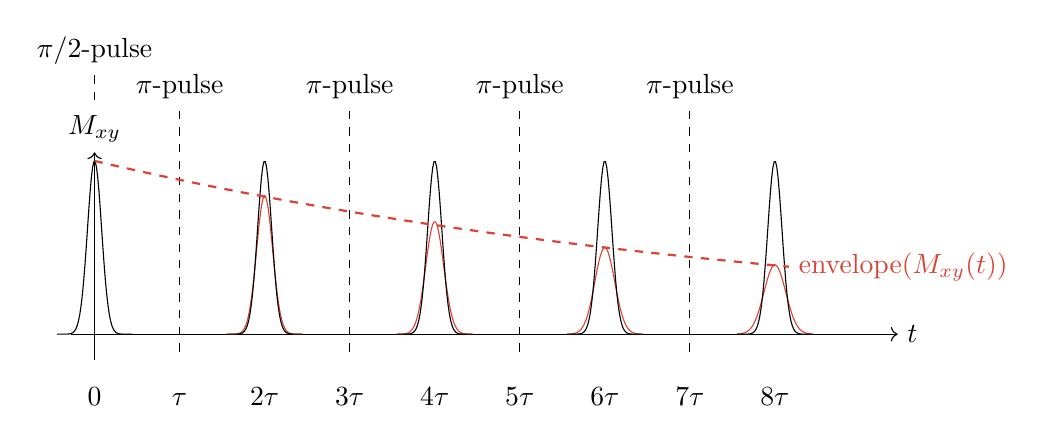
\begin{tikzpicture}[xscale=0.6, yscale=1.1]
    \draw[->] (-0.5,0) -- (17,0) node[right] {$t$};
    \draw[->] (0,-0.3) -- (0,2.1) node[above] {$M_{xy}$};

    \pgfmathsetmacro{\peakheight}{2.0}
    \pgfmathsetmacro{\sigpeak}{0.15}

    \node[anchor=north] at (0,-0.5) {$0$};

    \draw[dashed] (0,2.7) -- (0,3.0);
    \node[above] at (0,3.0) {$\pi/2$-pulse};

    \draw plot[domain=-0.8:0.8, samples=60]
    (\x, {\peakheight*exp(-(\x-0)^2/(2*\sigpeak^2))});

    \draw[dashed] (1.8,-0.2) -- (1.8,2.6);
    \node[above] at (1.8,2.6) {$\pi$-pulse};
    \node[anchor=north] at (1.8,-0.5) {$\vphantom{2}\tau$};

    \draw[Bzerocolor] plot[domain=2.8:4.4, samples=60]
    (\x, {1.6*exp(-(\x-3.6)^2/(2*0.17^2))});
    \draw plot[domain=2.8:4.4, samples=60]
    (\x, {\peakheight*exp(-(\x-3.6)^2/(2*\sigpeak^2))});
    \node[anchor=north] at (3.6,-0.5) {$2\tau$};

    \draw[dashed] (5.4,-0.2) -- (5.4,2.6);
    \node[above] at (5.4,2.6) {$\pi$-pulse};
    \node[anchor=north] at (5.4,-0.5) {$3\tau$};

    \draw[Bzerocolor] plot[domain=6.4:8.0, samples=60]
    (\x, {1.3*exp(-(\x-7.2)^2/(2*0.19^2))});
    \draw plot[domain=6.4:8.0, samples=60]
    (\x, {\peakheight*exp(-(\x-7.2)^2/(2*\sigpeak^2))});
    \node[anchor=north] at (7.2,-0.5) {$4\tau$};

    \draw[dashed] (9.0,-0.2) -- (9.0,2.6);
    \node[above] at (9.0,2.6) {$\pi$-pulse};
    \node[anchor=north] at (9.0,-0.5) {$5\tau$};

    \draw[Bzerocolor] plot[domain=10.0:11.6, samples=60]
    (\x, {1.0*exp(-(\x-10.8)^2/(2*0.21^2))});
    \draw plot[domain=10.0:11.6, samples=60]
    (\x, {\peakheight*exp(-(\x-10.8)^2/(2*\sigpeak^2))});
    \node[anchor=north] at (10.8,-0.5) {$6\tau$};

    \draw[dashed] (12.6,-0.2) -- (12.6,2.6);
    \node[above] at (12.6,2.6) {$\pi$-pulse};
    \node[anchor=north] at (12.6,-0.5) {$7\tau$};

    \draw[Bzerocolor] plot[domain=13.6:15.2, samples=60]
    (\x, {0.8*exp(-(\x-14.4)^2/(2*0.23^2))});
    \draw plot[domain=13.6:15.2, samples=60]
    (\x, {\peakheight*exp(-(\x-14.4)^2/(2*\sigpeak^2))});
    \node[anchor=north] at (14.4,-0.5) {$8\tau$};

    \draw[dashed, Bzerocolor, thick] plot[domain=0:14.7, samples=100]
    (\x, {2.0*exp(-(\x-0)/15.6)});
    \node[right, Bzerocolor] at (14.7, {2.0*exp(-(14.7-0)/15.6)})
    {$\text{envelope}(M_{xy}(t))$};
  \end{tikzpicture}
  \caption{Magnitude of a voltage proxy for $\vec M_{xy}$ versus time
    following a rotation of $\vec M$ into the transverse plane by a
    $\pi/2$ pulse. Periodic $\pi$ pulses with spacing $2 \tau$ cause
    spin echoes between each pulse as effects due to
    spatially-dependent Larmor frequencies are reversed and
    dephased magnetic moments are refocused. Without spin-spin effects,
    spin echoes can persist indefinitely (black). In reality,
    spin-spin effects cause
    irrecoverable loss of the transverse net magnetization across time
  (red) \cite{mel}.}
  \label{fig:spin_echo}
\end{figure}

This spin-spin effect is characterized by a time $T_2$ \cite{mel}:

\begin{equation}
  \text{envelope}(M_{xy}(t)) = M_{xy}(0) \cdot e^{- \frac{t}{T_2}}
  \label{eq:spin_spin_relaxation}
\end{equation}

A third constant $T_2^*$ is introduced to describe the decay time of
$M_{xy}$ considering spin-spin effects but without the refocusing
steps described in Figure \ref{fig:spin_echo}. All three constants
$T_1$, $T_2$, and $T_2^*$ can be related to each other, the nucleus's
gyromagnetic ratio $\gamma$,
and an effective average inhomogeneity in $|\vec B_0|$, $\Delta B_0$
\cite{mel, harris}:

\begin{equation}
  \frac{1}{T_2^*} = \frac{1}{T_2} + \frac{1}{T_1} + \gamma \Delta B_0
  \label{eq:const_relation}
\end{equation}

\section{Procedure}

\begin{figure}[H]
  \centering
  \resizebox{0.75\linewidth}{!}{%
    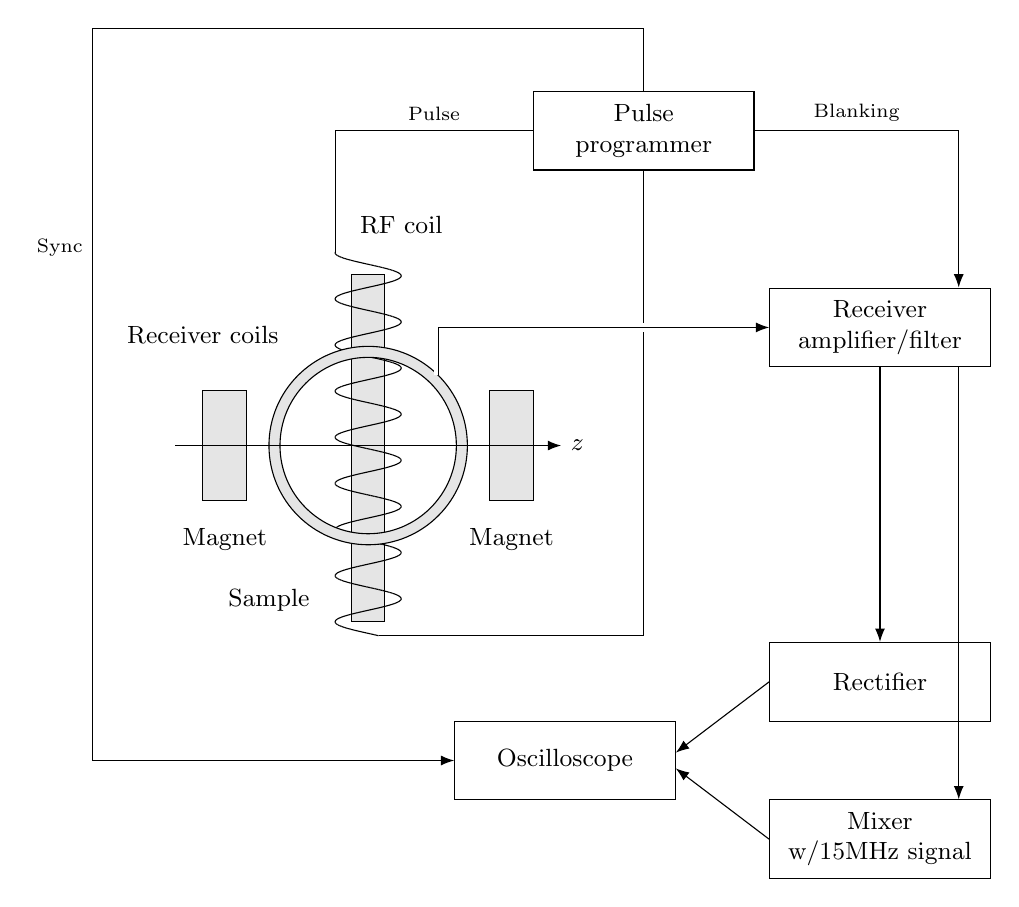
\begin{tikzpicture}[
        font=\small,
        >=Latex,
        block/.style={draw, align=center, minimum
        width=28mm, minimum height=10mm},
        sig/.style={-Latex},
        ctrl/.style={-Latex, dashed}
      ]

      % --- 2D Physical assembly
      \begin{scope}[shift={(-2.5,0)}, scale=0.7]

        % Sample - long vertical rectangle
        \draw[fill=gray!20, draw=black] (-0.3,-3.2)
        rectangle (0.3,3.1);
        \node at (-1.8,-2.8) {\small Sample};
        \coordinate (recvlead) at (0.3,-3);

        % RF coil - helix around sample
        \foreach \i in {3,4,...,418} {
          \pgfmathsetmacro{\angle}{50 + \i*7.2}
          \pgfmathsetmacro{\nextangle}{50 + (\i+1)*7.2}
          \pgfmathsetmacro{\z}{-3.5 + \i*0.01674}
          \pgfmathsetmacro{\znext}{-3.5 + (\i+1)*0.01674}
          \pgfmathsetmacro{\r}{0.6}
          \draw[black] ({\r*cos(\angle)}, \z) --
          ({\r*cos(\nextangle)}, \znext);
        }
        \coordinate (rflead1) at ({0.6*cos(50 + 3*7.2)}, -3.5 + 3*0.01674);
        \coordinate (rflead2) at ({0.6*cos(180)}, 3.5);
        \node at (0.6,4.0) {\small RF coil};

        % Helmholtz coils - annulus around sample
        \fill[gray!20, even odd rule] (0,0) circle (1.8) (0,0) circle (1.6);
        \draw[draw=black] (0,0) circle (1.8);
        \draw[draw=black] (0,0) circle (1.6);
        \node at (-3.0,2.0) {\small Receiver coils};
        \coordinate (helmholtzlead) at ({1.8*cos(45)},{1.8*sin(45)});

        % Left magnet - rectangle
        \draw[fill=gray!20, draw=black] (-3,-1) rectangle (-2.2,1);
        \node at (-2.6,-1.7) {\small Magnet};

        % Right magnet - rectangle
        \draw[fill=gray!20, draw=black] (2.2,-1) rectangle (3,1);
        \node at (2.6,-1.7) {\small Magnet};

        % z-axis through magnets
        \draw[->] (-3.5,0) -- (3.5,0) node[right] {$z$};

      \end{scope}

      % --- Electronic components
      \node[block] (pulseprog) at (1,4) {Pulse\\programmer};

      \node[block] (lc) at (4,1.5) {Receiver\\amplifier/filter};

      \node[block] (rectifier) at (4,-3) {Rectifier};

      \node[block] (mixer) at (4,-5) {Mixer \\ w/15MHz signal};

      \node[block] (scope) at (0,-4) {Oscilloscope};

      % --- Connections
      \draw (pulseprog.south) |- (rflead1)
      node[pos=0.25,right,font=\scriptsize] {};
      \draw (pulseprog.west) -| (rflead2)
      node[pos=0.25,above,font=\scriptsize] {Pulse};

      \draw[sig, white, line width=3pt] (helmholtzlead) |- (lc.west);
      \draw[sig] (helmholtzlead) |- (lc.west);

      \draw[sig] (pulseprog.east) -| ($(lc.north)+(1.0,0)$)
      node[pos=0.25,above,font=\scriptsize] {Blanking};

      \draw[sig] (pulseprog.north) -- (1,5.3) -- (-6,5.3) |- (scope.west)
      node[pos=0.15,left,font=\scriptsize] {Sync};

      \draw[sig] (lc.south) -- (rectifier.north);

      \draw[sig] ($(lc.south)+(1.0,0)$) -- ($(mixer.north)+(1.0,0)$);

      \draw[sig] (rectifier.west) -- ($(scope.east)+(0,0.1)$);

      \draw[sig] (mixer.west) -- ($(scope.east)+(0,-0.1)$);

    \end{tikzpicture}
  }
  \caption{Diagram of the experimental apparatus, including the
    sample, permanent magnets producing $\vec B_0$, RF coil supplying
    $\vec B_1$ according to a pulse programmer \cite{young, knight},
    receiver signal
    amplifier, mixer for measuring distance to resonance condition,
    and rectifier for obtaining the envelope of the transverse receiver
    coil signal \cite{boylestad}. Note that the $z$-axis defined by
    the permanent
    magnets is the same $z$-axis depicted in Figure
  \ref{fig:dipole_angular_momentum_3d}.}
  \label{fig:system_diagram}
\end{figure}

An experimental apparatus featuring a solution sample, input RF
coils, and detector coils is depicted in Figure
\ref{fig:system_diagram}. A sample is placed
in a static magnetic field $\vec B_0$ produced by two permanent
magnets, defining the $z$-axis and transverse plane depicted in Figure
\ref{fig:dipole_angular_momentum_3d}. An RF coil is wrapped around
the sample, used to produce the linearly-polarized field responsible
for providing the effective cicularly-polarized $\vec B_1$
\cite{young, knight}. Receiver coils
are placed with their axis in the transverse plane and orthogonal to the
RF coil. An induced current is measured in these as a result of the
the revolution of $\vec M_{xy}$--a process that creates an
oscillatory magnetic field with frequency $\omega_0$ and thus an
oscillatory magnetic flux through the coils \cite{young, knight}.

The voltage signal
from these receiver coils is filtered for a narrow band around
$\omega_0$ by a receiver module and then compared to the Larmor frequency of the
sample using a
$15$ MHz mixer, which produces a signal with frequency $\omega_0 -
\omega_1$ viewable
by a downstream oscilloscope \cite{boylestad}. For each sample, a
constant applied RF signal is produced and its frequency is varied until the
mixer signal has frequency zero, satisfying the resonance condition $\omega_0 =
\omega_1$. Once resonance is achieved, the RF signal is then shut off
and is later activated with controlled start times and durations using a
pulse programmer.

Following amplification, the output of the receiver coils also passes
through an AC-to-DC rectifier, allowing an oscilloscope to view a
voltage proxy for the magnitude of the transverse magnetization
vector, $M_{xy}$, as a function of time. Local maxima of this signal
with RF pulse duration correspond
to a completely transverse $\vec M_{xy}$, or to $\alpha = \pi / 2$.

Values of $T2^*$, $T_2$, and $T_1$ are obtained by samples of heavy
mineral oil, light mineral
oil, water, a 0.1 M CuSO$_4$ solution, a 1.0 M CuSO$_4$ solution, and
an unknown mineral oil. To assess consistency, a value of $\Delta
B_0$ is also obtained
independently using each sample's time constants.

\subsection{$T_2^*$ Measurement}

A coarse measurement of the aggregate transverse-component decay time
for each sample is obtained by providing an
$\alpha=\pi/2$ pulse using the pulse programmer and measuring the
time necessary for the transverse component to decay to $1/e$ of
its initial magnitude. Figure \ref{fig:scope_shot} depicts the
interval used to obtain this estimate for a sample of heavy mineral
oil. Values of $T_2^*$ per sample are organized in Table
\ref{tab:time_constants}.

\begin{figure}[H]
  \centering
  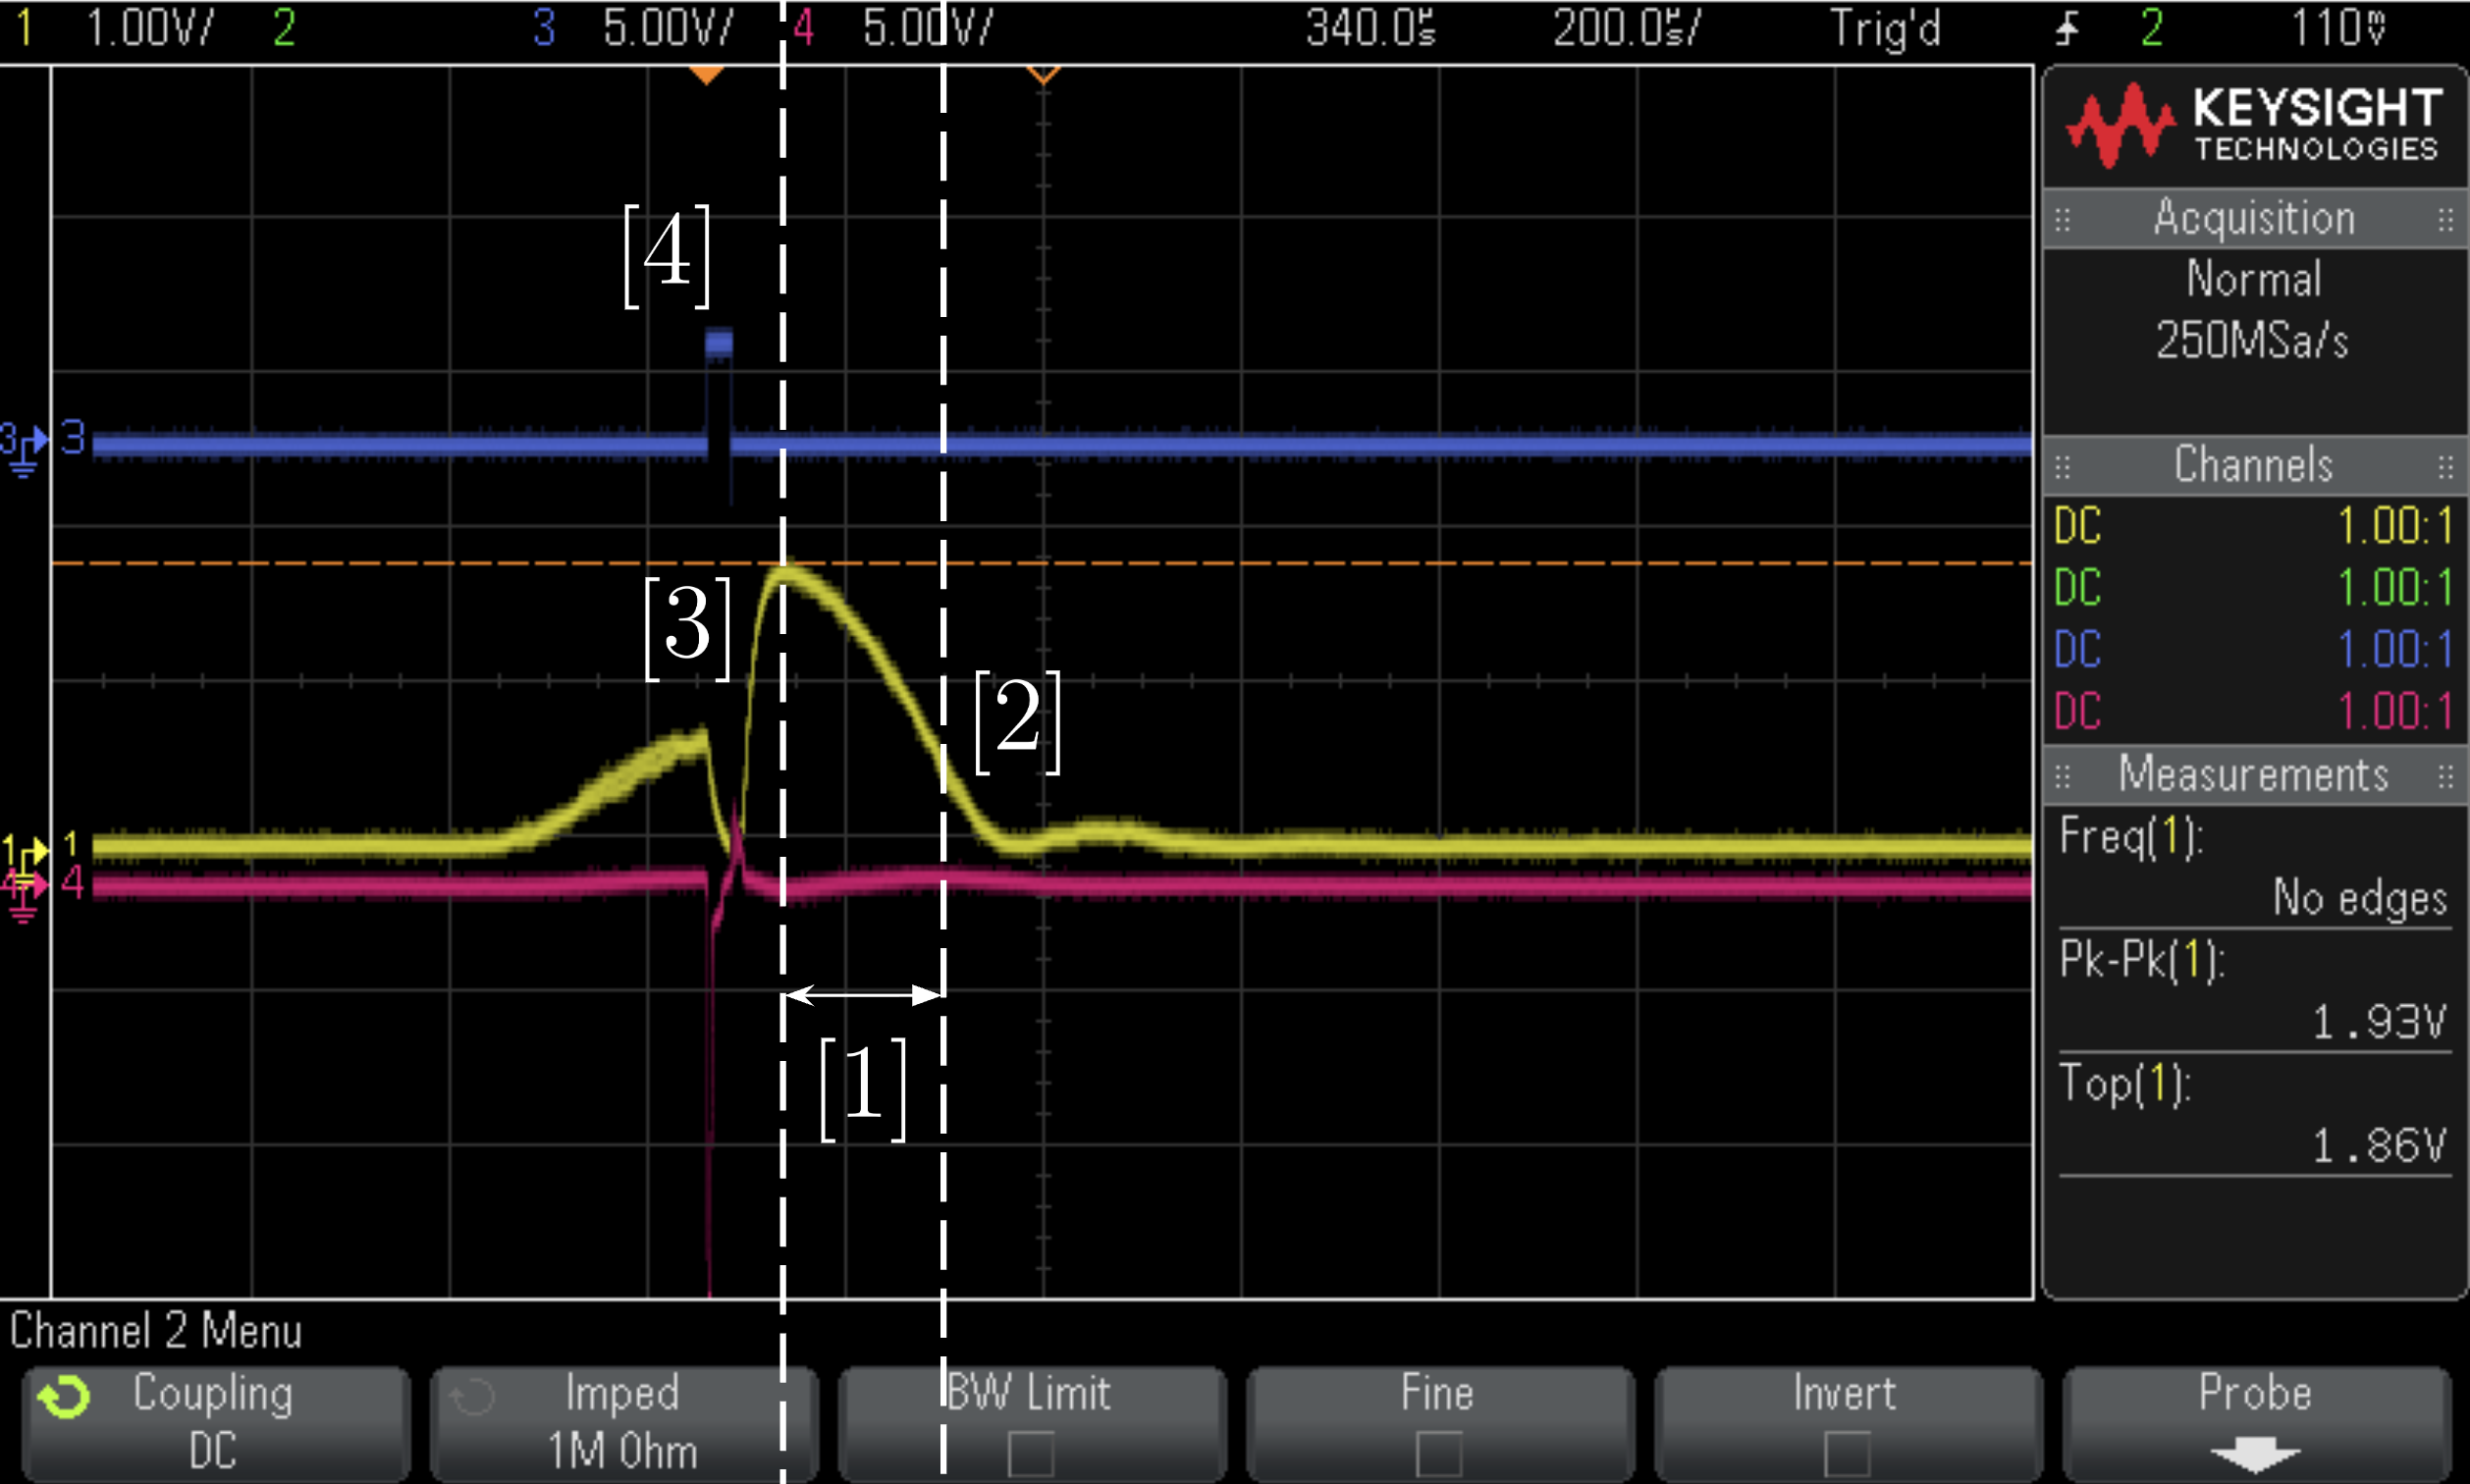
\includegraphics[width=0.8\textwidth]{../scope_shot.png}
  \caption{A screenshot of a single $\pi/2$ pulse [4] (blue) applied to a sample
    of heavy mineral oil, causing $\vec M$ to align itself with the
    transverse plane. The voltage proxy for $M_{xy}$ (yellow) is the
    envelope of the
    oscillatory signal collected from the receiver coils. This envelope
    exhibits a rising edge [3] during and shortly
    after the RF pulse, then a falling edge [2] as spin-spin and
    field-inhomogeneity effects cause the decay of $M_{xy}$ with
    time. The $T_2^*$ relaxation time [1] is estimated
    as the time taken by the pulse to decay to approximately $1/e$ of
  its initial value.}
  \label{fig:scope_shot}
\end{figure}

\subsection{$T_2$ Measurement}

A sample in the permanent magnetic field $\vec B_0$ is provided with
an initial $\alpha =\pi/2$ pulse, causing its net
magnetization vector $\vec M$ to lie in the transverse plane entirely. The
system is allowed
to experience spin-spin and field-inhomogeneity effects for a time
$\Delta t_0 = \tau$, at which point
an $\alpha=\pi$ pulse is provided. At time $2 \tau$, a spin echo is
observed, whose height $h_0$ along the voltage axis is measured using the
oscilloscope. Additional pulses are
provided at times $\Delta t_n = (2n + 1) \tau$ and spin heights
continue to be recorded until the
spin echo height disappears, yielding values $\set{h_0, h_1, h_2...}$
corresponding to echo times $\set{2\tau, 4\tau, 6\tau...}$.

$\tau$
is tuned per sample to achieve a reasonable
number of data points before the echo height decays to zero. The
decaying exponential function (\refeq{eq:spin_spin_relaxation})
is fit to this $h_n$-versus-$\Delta t_n$ data, yielding $T_2$ as its
characteristic time, depicted in \ref{fig:t2_fits}. Values of $T_2$
for samples are organized in Table
\ref{tab:time_constants}.

\subsection{$T_1$ Measurement}

A sample is again placed into $\vec B_0$, producing a $\vec M$-vector
initially at $\alpha = 0$. A $\alpha=\pi$ pulse is provided, causing
$\vec M$ to assume the
higher-energy anti-aligned state. The system is allowed to experience
spin-lattice relaxation for a time $\Delta t_1 = \xi$, at which point
a $\alpha=\pi/2$ pulse
is applied. The value of $M_{xy}$ following this $\pi/2$ pulse is equal to the
value of $M_z$ prior to the pulse, allowing for measurements of the
longitudinal height at time $\xi$. The system is then allowed to
relax entirely back to the $\alpha = 0$ state.

The process is repeated for times $\Delta t_n = \xi n$ until the
longitudinal magnitude decreases to zero then asymptotically increases
to a maximum value, yielding
heights $\set{h_1, h_2, h_3...}$ corresponding to measurement times
$\set{\xi, 2\xi, 3\xi...}$. Heights before the $h_i = 0$ criteria are negated
to reflect that $\vec M_z$ is anti-aligned with $\vec B_0$ prior to
the $\pi/2$ pulse used for measurement, and the exponential function
(\refeq{eq:spin_lattice_relaxation}) is fit to yield $T_1$ as its
characteristic time, depicted in Figure \ref{fig:t1_fits}. $T_1$ times
for samples are organized in Table \ref{tab:time_constants}.

\section{Results}

\begin{figure}[H]
  \centering
  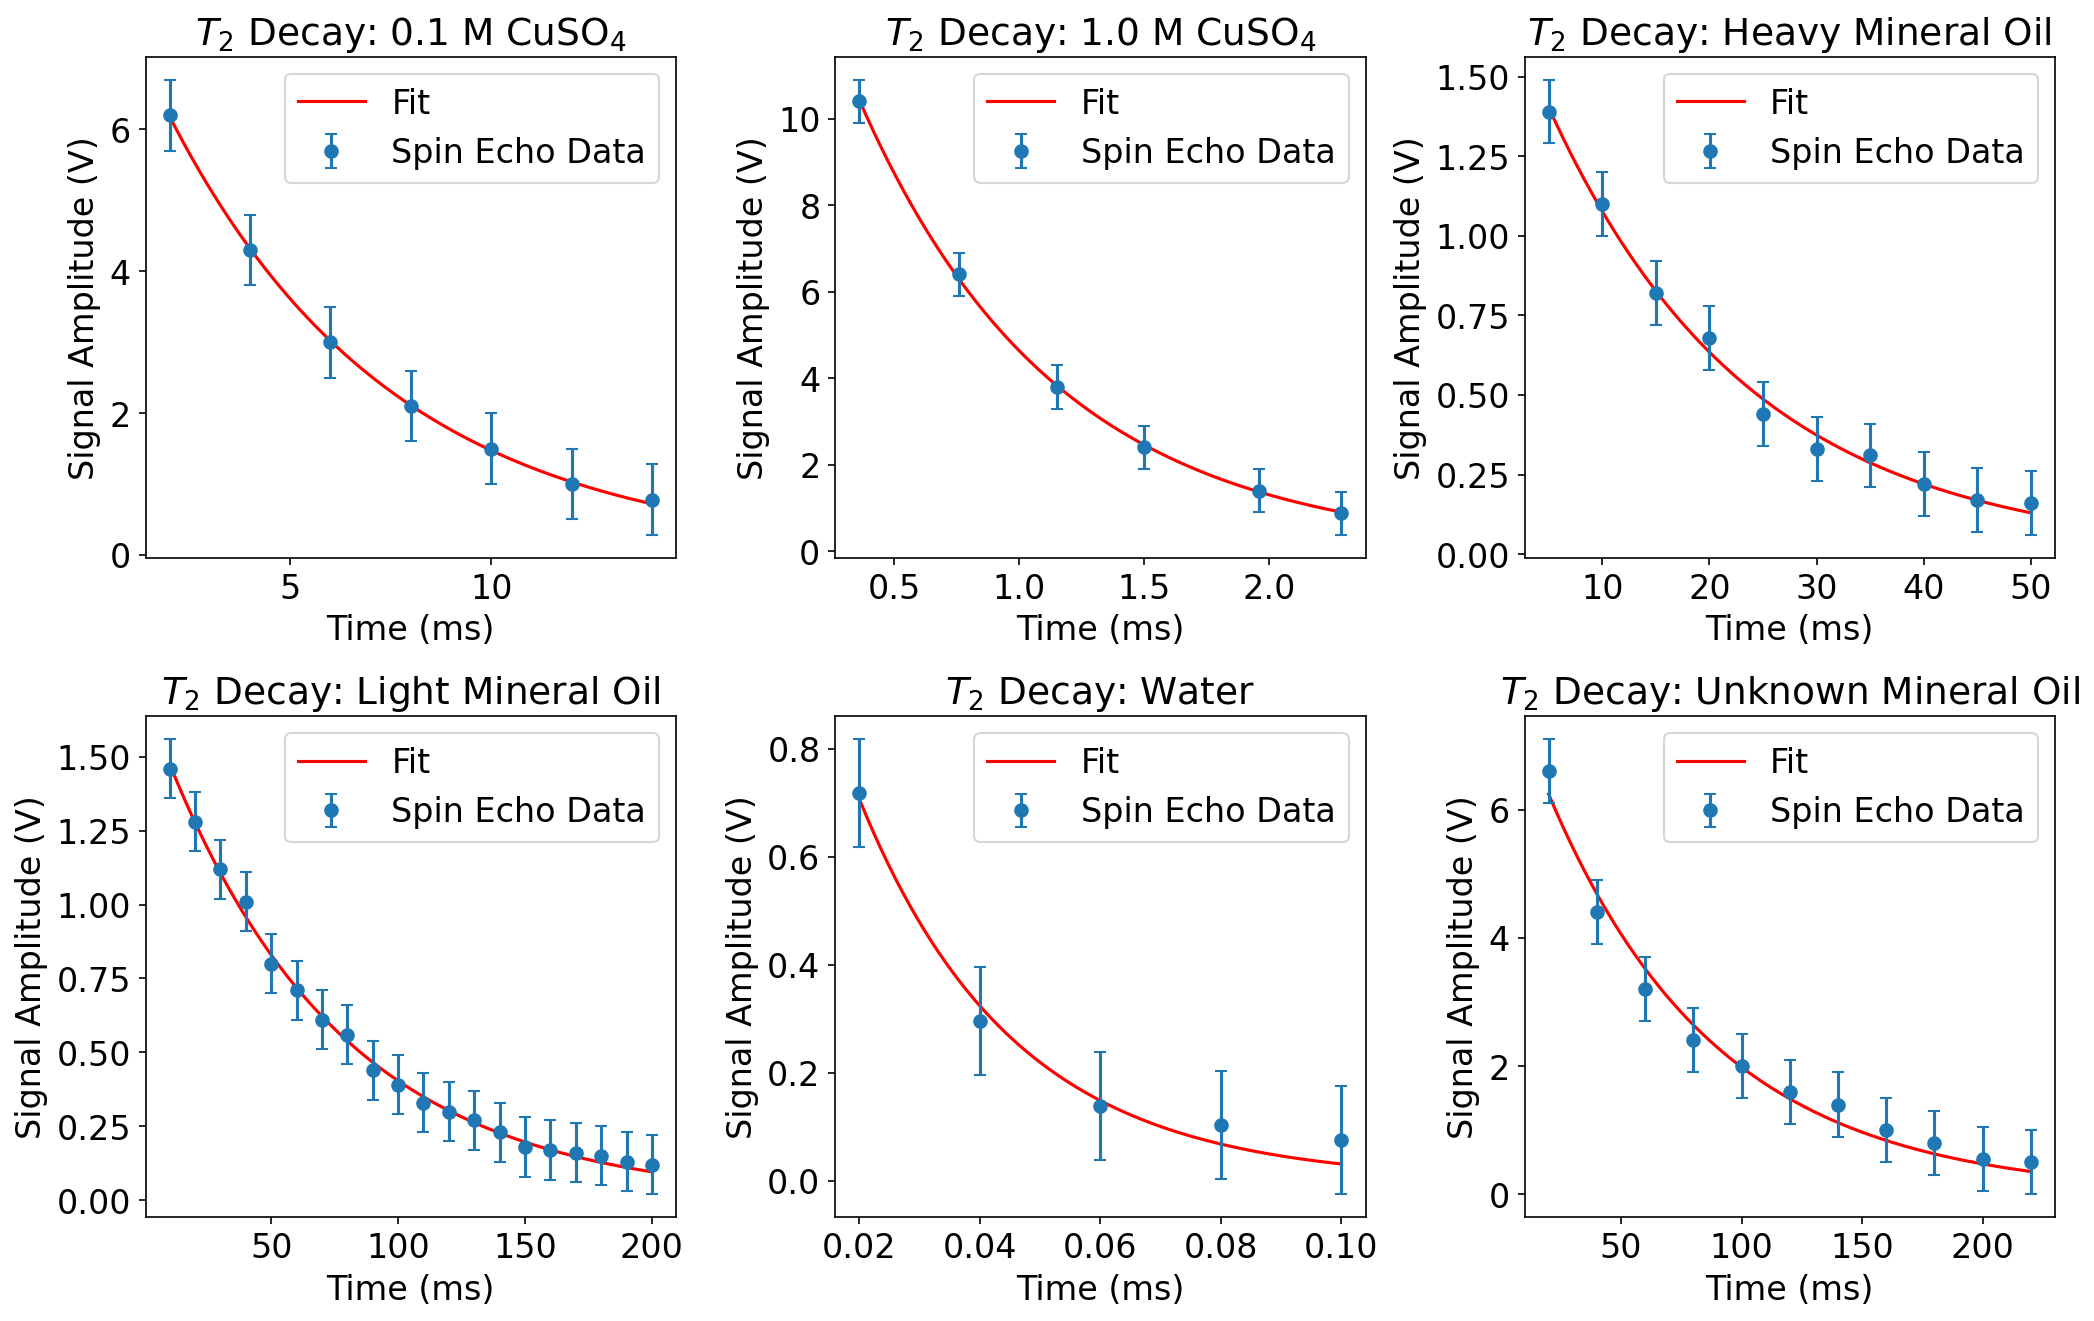
\includegraphics[width=\textwidth]{../output/t2_fits.pdf}
  \caption{Data points of spin echo heights versus echo time for each
    sample (blue) and the exponential decay curve of best fit (red) for
    each sample tested. The characteristic decay time of spin echo
  heights provides $T_2$.}
  \label{fig:t2_fits}
\end{figure}

\begin{figure}[H]
  \centering
  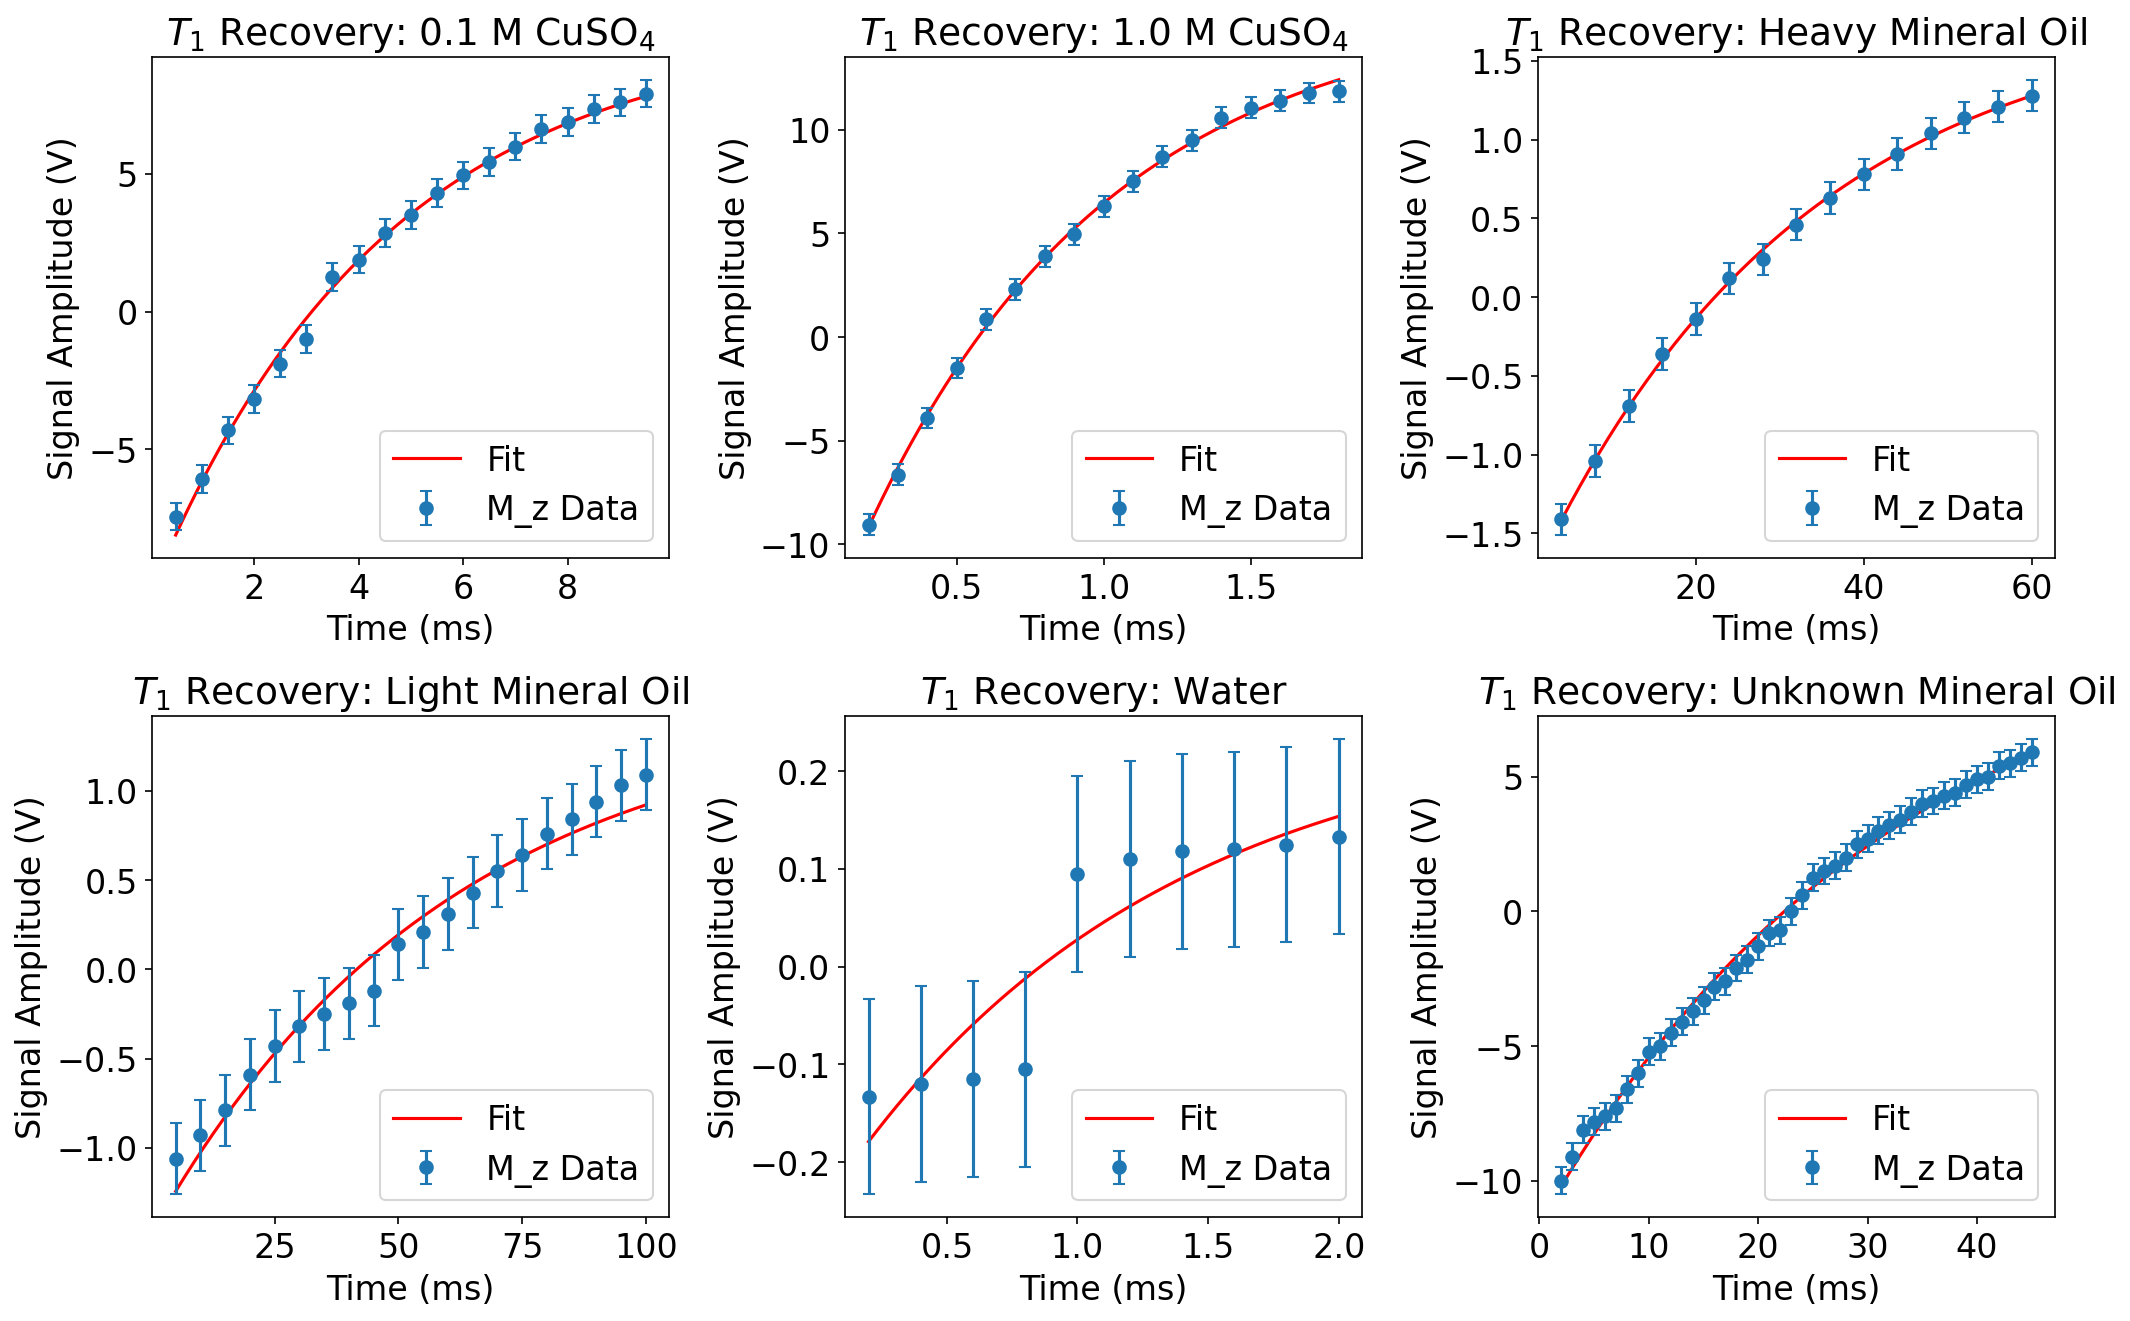
\includegraphics[width=\textwidth]{../output/t1_fits.pdf}
  \caption{Data points of $M_z$ magnitude (blue) versus the delay
    time of the $\pi/2$
    pulse used to bring $\vec M_z$ into the $xy$ plane for
    measurement via transverse receiver coils. Exponential recovery
    curves of best fit (red) provide $T_1$ as their characteristic
    time. Of note is the poor agreement between water's $T_1$ data points
    and the expected exponential recovery curve. Water has both a short
    relaxation time and a minimal longitudinal response to a resonant
    RF pulse, causing
    response peaks to be poorly distinguished from each other with
    unstable peak heights.
  }
  \label{fig:t1_fits}
\end{figure}

\begin{table}[H]
  \centering
  \begin{tabular}{lcccc}
    \hline
    Sample & $T_1$ (ms) & $T_2$ (ms) & $T_2^*$ (ms) ($\pm 15\%$) &
    $T_2^* / T_1$\\
    \hline
    0.1 M CuSO$_4$ & $4.48 \pm 0.09$ & $5.6 \pm 0.7$ & $0.28 \pm
    0.04$ & $0.062 \pm 0.010$ \\
    1.0 M CuSO$_4$ & $0.828 \pm 0.012$ & $0.79 \pm 0.07$ & $0.26 \pm
    0.04$ & $0.31 \pm 0.05$ \\
    Heavy Mineral Oil & $32.1 \pm 0.8$ & $18.9 \pm 1.9$ & $0.27 \pm
    0.04$ & $0.0084 \pm 0.0015$ \\
    Light Mineral Oil & $60.0 \pm 3.1$ & $69.0 \pm 5.0$ & N/A & N/A \\
    Water & $1.24 \pm 0.26$ & $0.026 \pm 0.007$ & N/A & N/A \\
    Unknown Mineral Oil & $32.29 \pm 0.34$ & $70.0 \pm 8.0$ & $0.29
    \pm 0.04$ & $0.0090 \pm 0.0013$ \\
    \hline
  \end{tabular}
  \caption{Experimental values for the three time constants $T_1$,
    $T_2$, and $T_2^*$, corresponding to spin-lattice effects,
    spin-spin effects, and net transverse decay (spin-lattice
    and field-inhomogeneity effects). Note that $15\%$ uncertainty
    bounds are applied to $T_2^*$ measurements to guarantee
    the capture of the point at which the transverse magnetization
    component decays to $1/e$ of its peak value following the
    $\pi/2$ pulse. Finally, a comparison of transverse decay time to
  longitudinal decay time ($T_2^* / T_1$) is included.}
  \label{tab:time_constants}
\end{table}

\begin{table}[H]
  \centering
  \begin{tabular}{lcc}
    \hline
    Sample & $\Delta B_0$ (T) & $\Delta B_0 / B_0$ \\
    \hline
    0.1 M CuSO$_4$ & $(1.18 \pm 0.21) \times 10^{-5}$ & $(3.6 \pm
    0.6) \times 10^{-5}$ \\
    1.0 M CuSO$_4$ & $(5.3 \pm 2.7) \times 10^{-6}$ & $(1.6 \pm 0.8)
    \times 10^{-5}$ \\
    Heavy Mineral Oil & $(1.35 \pm 0.21) \times 10^{-5}$ & $(4.1 \pm
    0.6) \times 10^{-5}$ \\
    Light Mineral Oil & N/A & N/A \\
    Water & N/A & N/A \\
    Unknown Mineral Oil & $(1.29 \pm 0.2) \times 10^{-5}$ & $(3.9
    \pm 0.6) \times 10^{-5}$ \\
    \hline
  \end{tabular}
  \caption{Experimental values for an effective average inhomogeneity
    $\Delta B_0$, computed for each sample using Table
    \ref{tab:time_constants}, Equation \ref{eq:const_relation}, and a
    measured $|\vec B_0|$ in the
    sample holder of $0.333 \pm 0.001$ T \cite{gyromag, mel}.
  Inhomogeneities are also expressed as a proportion relative to $|\vec B_0|$.}
  \label{tab:field_inhomogeneity}
\end{table}

\section{Discussion and Conclusion}

Experimental values of $T_1$, $T_2$, and $T_2^*$ are successfully obtained
for each sample, meeting the goal of characterizing the independent responses
of the longitudinal and transverse components of the net magnetization vector
to RF magnetic fields that meet resonance conditions.

Estimates of the average effective magnetic field inhomogeneity
computed using experimental time
constants from each sample produce values of $\Delta B_0$ that agree
with each other within $1 \sigma$ of each other, with the exception
of $\Delta B_0$ computed from the $1.0$ M CuSO$_4$ sample's time
constants--which agrees to within $2\sigma$ of the other values.
These inhomogeneities
are a few orders of magnitude smaller than the applied magnetic
field, which is consistent
with expectations.

Qualitatively, Table \ref{tab:field_inhomogeneity} suggests that solutions with
higher concentrations of solute exhibit faster overall relaxation
times (lower $T_1$ and $T_2$) in comparison with lower
concentrations. This is consistent
with intuition: larger numbers of excited nuclei result in more noisy
magnetic field fluctuations--
strengthening the spin-spin effect--while a larger number of
particles causes more efficient
energy transfer from the spins in excited states to a more dense
surrounding environment. Overall transverse relaxation effects also
appear to occur faster than longitudinal relaxation effects, apparent
in the small ratios between $T_2^*$ and $T_1$ for each sample.

This investigation of pulsed nuclear magnetic resonance is in direct
analogy with an experiment performed in PHYS 340 regarding the
torques experienced by a magnetic dipole in
a static vertical magnetic field and a smaller co-precessing magnetic
field. In this prior experiment, a macroscopic magnetic dipole with
an angular momentum
about the dipole axis was observed to precess about a vertical magnetic field
generated by a pair
of Helmholtz coils, analogous to nuclei precessing about $\vec B_0$
in this experiment. Toward the end of the PHYS 340 experiment, it was
demonstrated that rotating
a pair of magnets within the dipole's precessing frame caused a
displacement in the dipole's polar
angle with the $z$-axis, corresponding to a pulse through the RF coil
and a torque experienced about $\vec B_1$ in this pNMR situation.

The primary candidates for sources of discrepancy in this procedure is
the position of the sample in the magnetic field and the precision of tuning of
the RF frequencies to the resonance condition. The former would tend to reduce
transverse relaxation times, causing $\vec B_0$ to be more inhomogeneous
than expected. The latter is suspect because of the continuous nature of the
change in the mixer output as the RF frequency is varied; slightly
off-frequency RF pulses may cause mixer outputs to appear similar
to those of the correct frequency, causing relaxation times to be
lower as pulses become less effective at bringing the system into
higher-energy states.

\bibliographystyle{plain}
\bibliography{references}

\end{document}
